\chapter{Taxonomy}
\label{chap:intro}

In this chapter, we first briefly introduce the background of the research on human mobility as well as the corresponding visualization. Then we summarize the data source that are used to describe the human movement. After that, we summarize the general tasks of the human mobility analysis. At last, an overview of the whole survey is given.


\section{Background}

Movement is the fundamental characteristics of all the species, especially for the human-being, the movement range greatly represents the evolution history as well as the development of society and technology, while the movement patterns can also reflect the activities in relative small scale. Especially in the recent 150 years, with the rapid development of modern traffic, the movement pattern tends to be more diversified and complicated.  With the advanced sensing and location-based technology, more and more movement data are captured to describe human’s mobility. Nowadays, the movement data could precisely describe human activities in the urban, and raise an increasing attention of researchers in different research domains like urbanology, meteorology, sociology and economics. 

However, the analysis of the movement data is difficult, in addition to the increasing data size, the movement data has spatial-temporal features which is independent to other attributes. And the movement patterns also differ from time and region. Besides, some reasoning tasks from the data are also require domain knowledge, which needs the involvement of domain expert. 

Visualization provides the methods that leverage the distinct capabilities of machine and human for the exploration tasks. Hundreds of years ago, the visualization to human movement has been designed that enable human to understand the movement patterns. 

A classic case of the mobility visualization is Napoleon’s campaign to Russia(Figure) which is depicted by French civil engineer Charles Joseph Minard. This well designed figure not only the present the spatial-temporal features of the marching route, but also the moving directions, number of troops as well as the temperature.  


\begin{figure}[!htb]
  \centering
  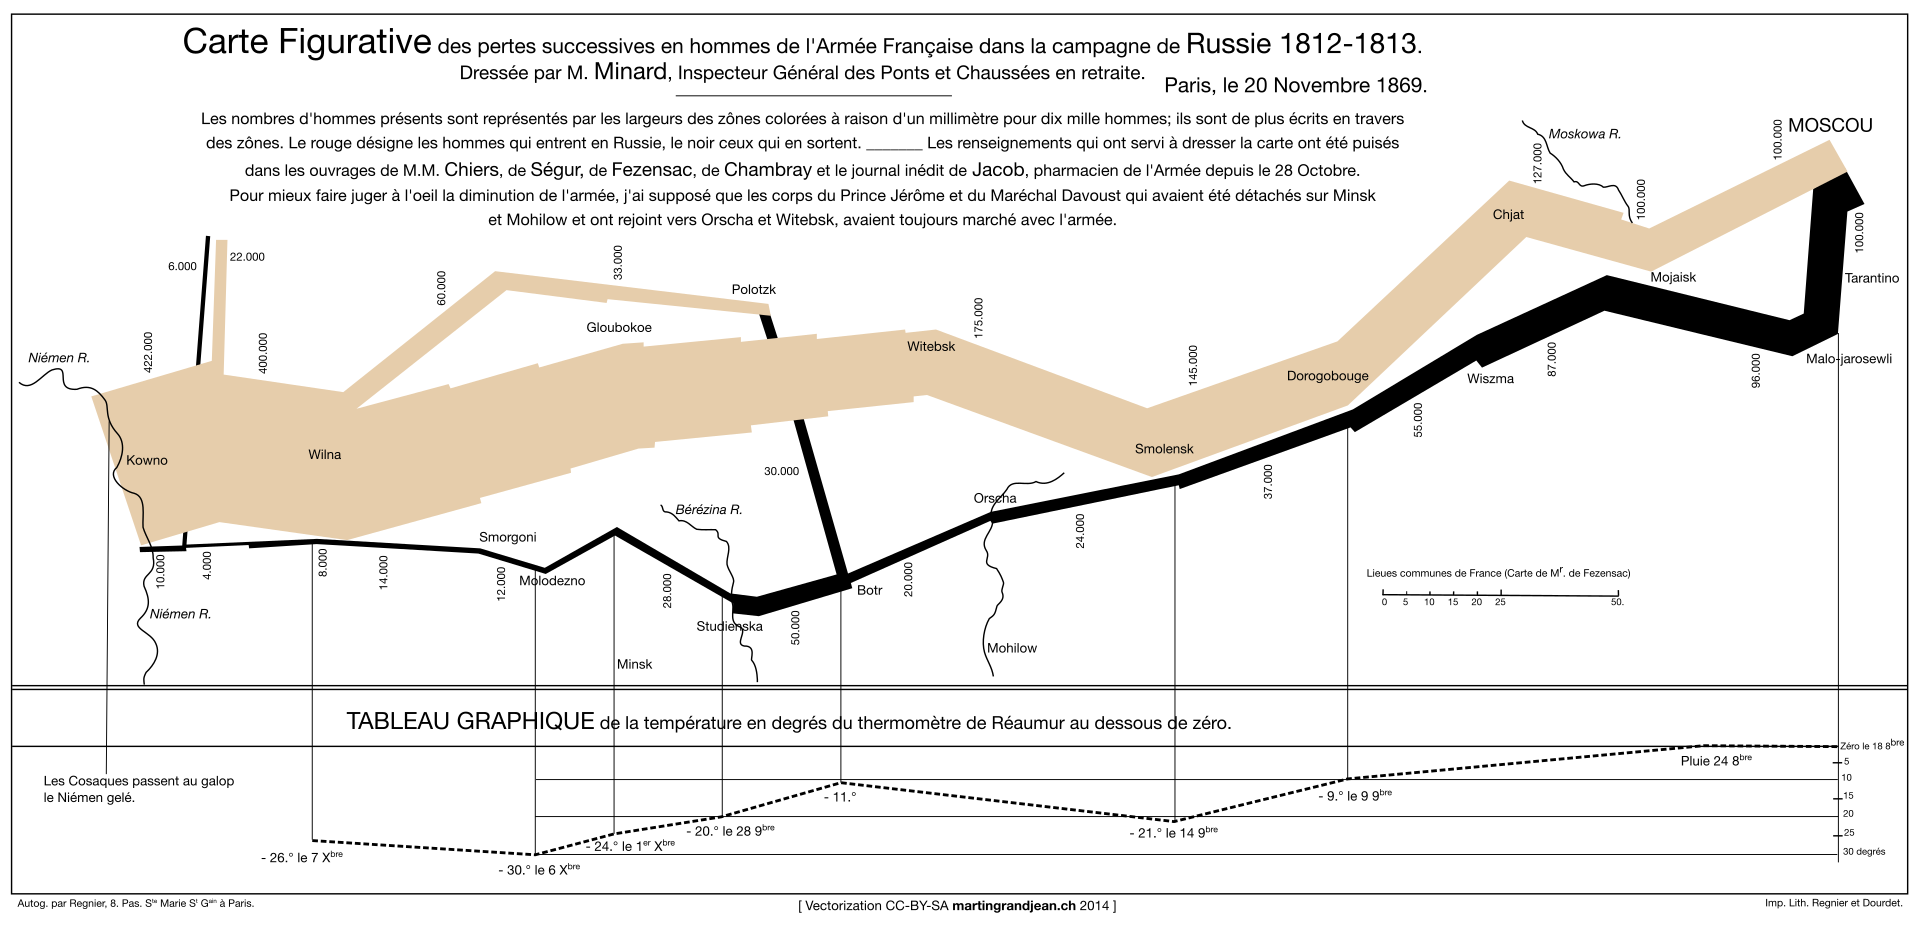
\includegraphics[width = 400px]{figures/Napoleon_war.png}
  \caption{Charles Minard's map of Napoleon’s campaign to Russia of 1812. The band illustrates the marching route from Kaunas to Moscow. The position on the figure present the relative position of geo-map. The band width illustrates the troop number and the color indicates the directions of departure and withdraw. }
  \label{fig:napoleon}
\end{figure}

With the rapid development of computer techniques, the more advanced visual analytics are designed based on powerful computing capability as well as the efficient algorithms. Instead the effectiveness of visual design, the modern visual analytics also focus on the how to bridge the gap between users and computers. As for the exploration itself, the interactive analysis on complicated tasks should be considered. 

\section{Data and tasks}



\section{Overview}


The whole survey is organized as follows: 

Chapter 2 introduces the existed taxonomies which has been widely accepted in specific domain. Generally, these taxonomies are designed based the application, data feature or analytics technology.

Chapter 3 focus on the data modeling methods for the mobility analysis from a new perspective. We found all the previous work of mobility analysis model the movement data into three ways, spatial-based points, origin-destination and trajectory. These model methods usually highly correspond to the characters of data and research problems. 

Chapter 4 focus on the different stages of visual analytics pipeline. We mainly discuss the techniques used in different stages. 

Chapter 5 introduce the detail applications and discuss how problem of different application can be addressed by the specific modeling methods and techniques. 

Chapter 6 makes a conclusion and discusses the future research directions.

